%%% File encoding: UTF-8
%%% äöüÄÖÜß  <-- keine deutschen Umlaute hier? UTF-faehigen Editor verwenden!

%%% Magic Comments zum Setzen der korrekten Parameter in kompatiblen IDEs
% !TeX encoding = utf8
% !TeX program = pdflatex 
% !TeX spellcheck = de_DE
% !BIB program = biber

\documentclass[master,german,smartquotes]{hgbthesis}
% Zulässige Optionen in [..]: 
%   Typ der Arbeit: diploma, master (default), bachelor, internship
%   Hauptsprache: german (default), english
%		smartquotes: zur vereinfachten Eingabe von Hochkommas (nur "...")
%%%----------------------------------------------------------

\RequirePackage[utf8]{inputenc}		% bei der Verw. von lualatex oder xelatex entfernen!

\graphicspath{{images/}}    % Verzeichnis mit Bildern und Grafiken
\logofile{logo}							% Logo-Datei = images/logo.pdf (\logofile{}, wenn kein Logo gewünscht)
\bibliography{references}  	% Biblatex-Literaturdatei (references.bib)

%%%----------------------------------------------------------
% Angaben für die Titelei (Titelseite, Erklärung etc.)
%%%----------------------------------------------------------

%%% Einträge für ALLE Arbeiten: -----------------------------
\title{MiniJava-Compiler für WebAssembly auf Basis von ANTLR und Kotlin}
\author{Stefan Schöberl, BSc}

\programtype{Fachhochschul-Masterstudiengang}

\programname{Software Engineering}
\placeofstudy{Hagenberg}
\dateofsubmission{2020}{06}{30}	% {YYYY}{MM}{DD}

\advisor{FH-Prof. DI Dr. Heinz Dobler}	% optional

%\strictlicense		%%% restrictive license instead of Creative Commons (discouraged!)

%%%----------------------------------------------------------
\begin{document}
%%%----------------------------------------------------------

%%%----------------------------------------------------------
\frontmatter                    % Titelei (röm. Seitenzahlen)
%%%----------------------------------------------------------

\maketitle
\tableofcontents

\chapter{Kurzfassung}

WebAssembly ist eine neue Technologie, die mittlerweile in aktuellen Browsern integriert ist. Seit Dezember 2019 ist WebAssembly ein offizieller Web"=Stanard des W3C. WebAssembly verwendet einen eigenen Bytecode, dessen Ausführungsmodell auf einer virtuellen Kellermaschine basiert und verspricht schnellere Ladezeiten und bessere Performanz als beispielsweise JavaScript. Dadurch ist es möglich, andere Programmiersprachen ohne Transpiler im Web einzusetzen. Dafür sind allerdings Compiler notwendig, die für WebAssembly Bytecode erzeugen können. Java Applets verfolgten einen ähnlichen Ansatz, indem sie die Java Virtual Machine (JVM) im Browser einsetzten, jedoch wird diese Technologie mittlerweile nicht mehr in aktuellen Browsern unterstützt.

Diese Masterarbeit befasst sich mit der Entwicklung eines Compilers für MiniJava, einer Teilmenge der von Java. Dabei wird gezeigt, wie Sprachkonstrukte dieser Programmiersprache auf WebAssembly abgebildet werden können. Weiters wird auf das zur Ausführung notwendige Laufzeitsystem eingegangen. Eine Besonderheit dabei ist, dass Objekte in MiniJava auf JavaScript"=Objekte abgebildet werden, dadurch ist beispielsweise im Browser ein direkter DOM"=Zugriff möglich. Die praktische Anwendung des geschaffenen Compilers wird anhand einer Demo"=Anwendung im Browser, einem Fibonacci"=Rechner, demonstriert. Diese Anwendung wurde, bis auf generische notwendige Skripte zum Laden der Anwendung, zur Gänze in MiniJava implementiert.

In dieser Masterarbeit wird damit eine Möglichkeit aufgezeigt, wie neue Programmiersprachen auf Basis von WebAssembly in das Web gebracht werden können.

\chapter{Abstract}


\begin{english}
WebAssembly is a new technology, which is supported in current browsers by now. Since december 2019 WebAssembly is an official Web standard of the W3C. Web\-As\-sem\-bly uses its own bytcode, whose execution model is based on a stack machine and promises faster loading times and better performance than JavaScript, for example. Thus it is possible, to bring other programming languages without a transpiler to the Web. However, compilers are necessary, that can produce bytecode for WebAssembly. Java Applets were based on a similar approach by using the Java virtual machine (JVM) within the browser, but this technology is no longer supported in current browsers.

This master's thesis deals with the development of a compiler for MiniJava, a subset of Java. It is shown how features of this programming language will be mapped to WebAssembly. In addition, the runtime system required for execution is described. A special feature is the direct mapping of objects in MiniJava to JavaScript objects. This enables direct DOM access in the browser, for example. The practical use of the created compiler is demonstrated with a browser demo application, which is a Fibonacci calculator. This application was implemented entirely in MiniJava, except for some generic scripts required to load the application.

This master's thesis shows an approach, how new programming languages can be brought to the Web based on WebAssembly.
\end{english}


%%%----------------------------------------------------------
\mainmatter          % Hauptteil (ab hier arab. Seitenzahlen)
%%%----------------------------------------------------------

\chapter{Einleitung}

\section{Motivation}

WebAssembly \cite{WebAssemblyWebsite} ist eine relativ neue (2017) Technologie mit dem Ziel, eine sprachunabhängige Plattform fürs Web zu schaffen. Da nur JavaScript von Browsern unterstützt wird, ist man auf diese Sprache beschränkt. Früher konnte man auch Java-Applets mit Java entwickeln, die direkt im Browser ausgeführt werden konnten. Aktuelle Browserversionen unterstützen diese Technologie mittlerweile nicht mehr und Oracle stellt ebenfalls die Unterstützung ein \cite{OracleJavaSESupportRoadmap}.

Anders sieht es bei Sprachen wie beispielsweise TypeScript aus: Um diese im Browser auszuführen, muss der Quelltext zunächst mit einem Transpiler nach JavaScript übersetzt werden. Anschließend muss der resultierende JavaScript-Quelltext vom Browser zur Laufzeit interpretiert werden \cite{TypeScript}.

WebAssembly verfolgt einen alternativen Ansatz, in dem eine Laufzeitumgebung in Form eines Kellerautomaten vom Browser zur Verfügung gestellt wird, so ähnlich wie früher die Java Virtual Machine mit Java-Applets. Über eine JavaScript-Schnittstelle können zur Laufzeit Module geladen werden, die im Kellerautomat ausgeführt werden. Module müssen in Form eines eigenen Bytecodes zur Verfügung stehen.

Ein geeigneter Compiler kann nun eine (beliebige) Programmiersprache in diesen Bytecode übersetzen. So ist ein Konvertieren des Quelltextes über einen Transpiler nicht mehr notwendig.

WebAssembly ist nicht als Alternative, sondern als Ergänzung zu JavaScript zu sehen. Ein Ziel ist, bestehenden Quelltext wiederverwenden zu können, auch wenn dieser in einer anderen Programmiersprache geschrieben wurde. Mit JavaScript werden die einzelnen Komponenten anschließend miteinander verbunden.

Damit dieses Ziel erreicht werden kann, müssen Compiler verschiedener Sprachen in der Lage sein, WebAssembly-Bytecode zu erzeugen.

\section{Problemstellung}

Die Problemstellung für diese Masterarbeit lässt sich in folgende Fragen aufteilen:

\begin{enumerate}
	\item Was ist WebAssembly, welche Möglichkeiten bietet WebAssembly und welche Einschränkungen gibt es?
	\item Wie kann ein Compiler, der eine Programmiersprache nach WebAssembly übersetzt, implementiert und getestet werden?
	\item Wie werden typische Sprachkonstrukte einer Programmiersprache auf Web\-As\-sem\-bly-Befehle abgebildet?
	\item Wie wird die Schnittstelle zum Browser entworfen und auf welche Aspekte muss dabei geachtet werden?
\end{enumerate}

\section{Ziele}

Die Fragen der Problemstellung sollen auf auf Basis einer praktischen Implementierung beantwortet werden.

Ziel ist es, einen Compiler zu entwickeln, der MiniJava (eine Teilmenge von Java) nach WebAssembly übersetzt. Die Eingabe ist MiniJava-Quelltext, die Ausgabe ein WebAssembly-Modul samt Laufzeitsystem für JavaScript. Der gesamte Compiler wird in Kotlin entwickelt. Das Compiler-Frontend (Scanner und Parser) wird mit ANTLR 4 generiert.

Schlussendlich soll es möglich sein, in MiniJava eine kleine typische Web-Anwendung zu entwickeln.

Weiters wird eine minimale Standardbibliothek entworfen. Diese stellt essentielle Schnittstellen für die Konsole und den DOM-Zugriff zur Verfügung.

Es gibt bereits einige Technologien, die auf WebAssembly aufbauen. Auf drei ausgewählte wird in dieser Arbeit kurz eingangen:
\begin{itemize}
    \item Emscripten \cite{Emscripten} für C und C++
    \item Rust \cite{RustWasmWebsite}
    \item Blazor \cite{Blazor} 
\end{itemize}

Beim Einsatz von Emscripten und Rust ist im C/C++/Rust-Quelltext ersichtlich, dass JavaScript oder WebAssembly im Hintergrund verwendet wird. Bei Emscripten sind das beispielsweise Einschlüsse von JavaScript-Fragmenten oder bei Rust müssen spezielle Attribute eingefügt werden. Blazor ist ein Framework zum Entwickeln von Web-Anwendungen und bietet somit eine Komplettlösung an. Hier kann bestehender C\#{}-Code unter gewissen Voraussetzungen wiederverwendet werden.

Mit MiniJava soll ein alternativer Ansatz versucht werden, eine (neue) Programmiersprache ins Web über WebAssembly zu bringen: MiniJava-Quelltext soll im Unterschied zu Emscripten und Rust keine Hinweise darauf enthalten, dass der kompilierte Quelltext schlussendlich mit JavaScript und WebAssembly interagiert. Es soll mit MiniJava auch kein Framework aufgebaut werden wie bei Blazor. Weiters sollen Objekte in MiniJava 1:1 auf JavaScript-Objekte abgebildet werden, dadurch soll beispielsweise direkter Zugriff auf den DOM ermöglicht werden. Dieser Ansatz findet sich so in keiner der drei Technologien. Schnittstellen zur Laufzeitumgebung werden in MiniJava über native Methoden umgesetzt. Dieses Sprachkonstrukt ist aus Java bekannt.

\section{Aufbau der Arbeit}

Die Arbeit ist in aufeinander aufbauende Kapitel gegliedert:
\begin{enumerate}
    \setcounter{enumi}{1}
    \item \emph{Technische Grundlagen:} Die Implementierung dieser Arbeit baut auf diversen Technologien auf. In diesem Kapitel werden die für diese Arbeit notwendigen Technologien beschrieben. Ein besonderer Fokus liegt hier auf WebAssembly und ANTLR, es wird aber auch auf diverse Hilfstechnologien eingegangen. Zum Schluss werden drei aktuelle Technologien im Detail betrachtet, die bereits WebAssembly-Unterstützung anbieten.
    \item \emph{Anforderungen an den Compiler und das Laufzeitsystem:} In diesem Kapitel wird die Programmiersprache MiniJava vorgestellt. Dieses Kapitel ist als Art Anforderungskatalog für den Compiler und das Laufzeitsystem zu sehen.
    \item \emph{Codegenerierung für WebAssembly:} In diesem Kapitel wird gezeigt, wie aus Mi\-ni\-Ja\-va-Quell\-text ein WebAssembly-Modul erzeugt wird. Dabei wird insbesonders gezeigt, wie die Sprachkonstrukte auf WebAssembly abgebildet werden. 
    \item \emph{Integration mit JavaScript:} Das erzeugte WebAssembly-Modul benötigt zur Ausführung noch ein Laufzeitsystem, auf dieses wird in diesem Kapitel eingangen. Das Laufzeitsystem ist in JavaScript implementiert. Weiters wird vom Compiler auch JavaScript-Quelltext generiert, um das Modul ausführen zu können.
    \item \emph{Testen des Compilers und Integration des Compilers in Gradle:} Um eine korrekte Funktion des Compilers zu gewährleisten, muss er getestet werden. Auf diesen Aspekt wird in diesem Kapitel im Detail eingangen. Weiters wird gezeigt, wie der Compiler in Gradle integriert werden kann, um ihn so in eigenen Projekten verwenden zu können. Diese Integration wird anhand einer Konsolenanwendung veranschaulicht.
    \item \emph{Demo-Anwendungen im Browser:} In diesem Kapitel wird ein Fibonacci-Rechner als Web-Anwendung präsentiert, um die praktische Anwendung von MiniJava zu demonstrieren. Weiters wird hier kurz auf die Standardbibliothek für DOM-Zugriffe eingangen.
\end{enumerate}

Zum Schluss werden die Ergebnisse der Arbeit zusammengefasst und es wird ein Ausblick auf mögliche Erweiterungen gegeben.

\pagebreak
\section{Architektur des Gesamtsystems}

Um zu Beginn einen Überblick zu geben, wird in Abbildung \ref{fig:architecture} die Architektur des Gesamtsystems dargestellt. Nachfolgend werden die wichtigsten Vorgänge beschrieben:

\begin{enumerate}
    \item Die Eingaben des Compilers sind MiniJava- und Ja\-va\-Script-Quelltexte. Die Ja\-va\-Script-Quelltexte enthalten die Implementierung nativer Methoden.
    \item Die MiniJava-Quelltexte werden vom generierten Scanner und Parser analysiert und in Syntaxbäume umgewandelt. Diese Syntaxbäume werden mit \emph{Visitors} und Codegeneratoren zu einem WebAssembly-Modul (als Datenstruktur im Arbeitsspeicher) verarbeitet. Dabei werden ebenfalls Metainformationen über den Mi\-ni\-Ja\-va-Quelltext gesammelt.
    \item Der Paketgenerator erzeugt aus dem Modul, den Meta-Informationen und den JavaScript-Quelltexten ein Paket. Ein Paket ist ein Verzeichnis mit einer definierten Struktur. Darin ist unter anderem das WebAssembly-Modul als Datei enthalten.
    \item Das Laufzeitsystem lädt in der Laufzeitumgebung das Paket, dabei wird die Web\-As\-sem\-bly-API eingesetzt. Daraus entsteht ein lauffähiges Modul.
    \item Nun kann das Modul gestartet werden und Ausgaben auf der Konsole oder visuell im DOM erzeugen.
\end{enumerate}


\begin{figure}[]
    \centering
    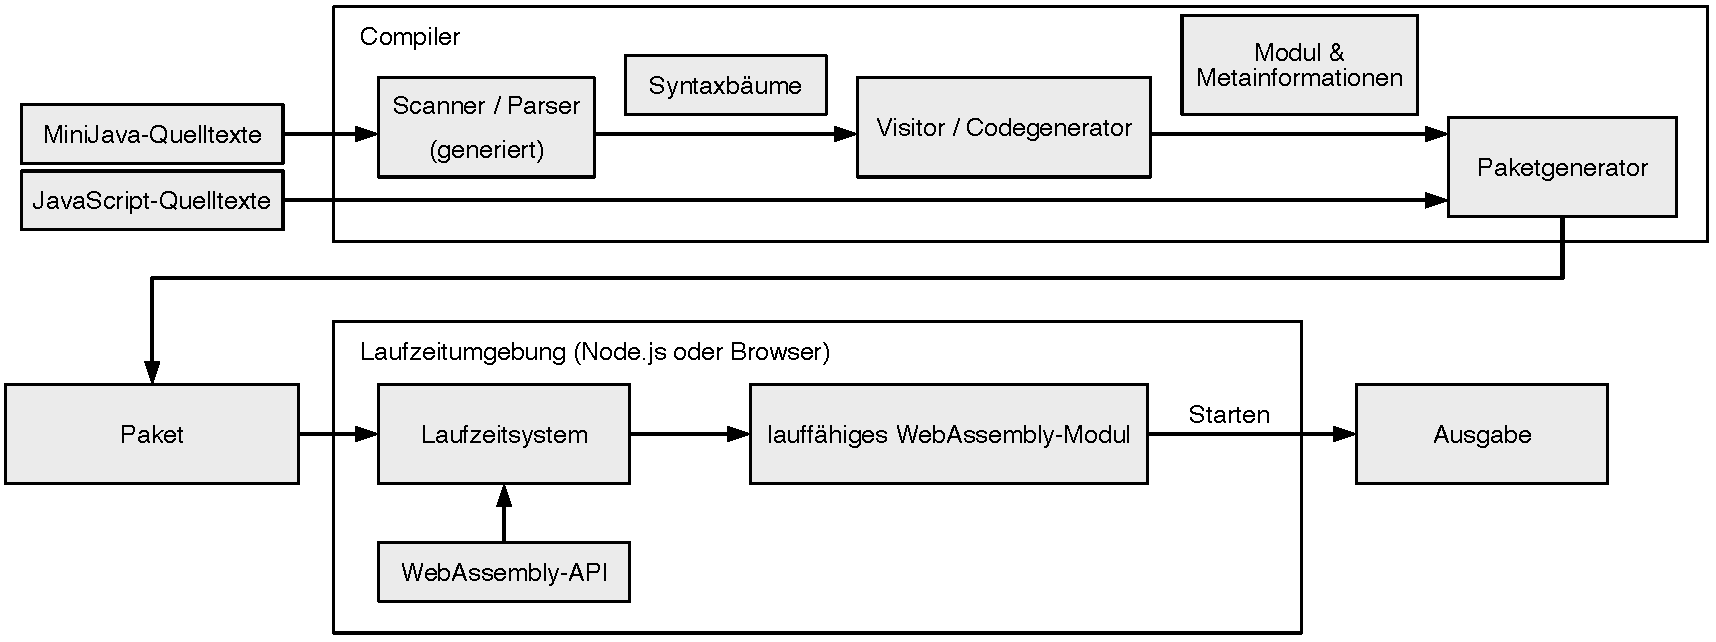
\includegraphics[width=\textwidth]{einleitung/architecture}
    \caption{Architektur des Gesamtsystems}
    \label{fig:architecture}
\end{figure}

\section{Verweis auf Quelltext}
Der Quellcode des gesamten Compilers und der Demo-Beispiele steht auf GitHub zum Download zur Verfügung: \url{https://github.com/stefanschoeberl/TODO}

\chapter{Zusammenfassung}

In diesem Kapitel werden die Ergebnisse der Arbeit zusammengefasst und es wird ein Ausblick auf mögliche Erweiterungen des MiniJava-Compilers und alternative Ansätze gegeben. Zum Schluss gebe ich einen Einblick auf meine persönlichen Erfahrungen während der Entwicklung des Compilers.

\section{Ergebnisse}

Alle vier Fragen der Problemstellung wurden in dieser Arbeit beantwortet:
\begin{enumerate}
	\item Was ist WebAssembly, welche Möglichkeiten bietet WebAssembly und welche Einschränkungen gibt es?
	\item Wie kann ein Compiler, der eine Programmiersprache nach WebAssembly übersetzt, implementiert und getestet werden?
	\item Wie werden typische Sprachkonstrukte einer Programmiersprache auf Web\-Assem\-bly-Befehle abgebildet?
	\item Wie wird die Schnittstelle zum Browser entworfen und auf welche Aspekte muss dabei geachtet werden?
\end{enumerate}

Zu Beginn wurde im \ref{cha:Technische-Grundlagen} Kapitel (Technischen Grundlagen) WebAssembly als Technologie detailliert behandelt. Weiters wurden drei Technolgien (Emscripten, Rust und Blazor) vorgestellt, die bereits auf WebAssembly aufbauen. Dabei wurden auch einige Einschränkungen von WebAssembly dargestellt, beispielsweise kann nicht zu jeder beliebigen Instruktion gesprungen werden, da Sprünge strukturiert sein müssen. Weiters wurde ein Ausblick auf weitere Entwicklungen von WebAssembly gegeben. In den technischen Grundlagen wurden außerdem diverse Technologien behandelt, die für die Implementierung notwendig sind, wie beispielsweise ANTLR und Kotlin. Hier wurde die erste Frage der Problemstellung beantwortet

In Kapitel \ref{cha:MiniJava} wurde die Programmiersprache MiniJava vorgestellt, für die ein Compiler entwickelt wurde. Weiters wurde auf die Anforderungen an das Laufzeitsystem eingegangen.

Die zweite Frage wurde in den Kapiteln \ref{cha:Codegenerierung-für-WebAssembly} und \ref{cha:Testen-des-Compilers} beantwortet. Hier wurde gezeigt, wie die Sprachkonstrukte aus MiniJava auf WebAssembly-Bytecode abgebildet werden und wie der Compiler getestet wird. JavaScript-Aspekte, die zur Laufzeit notwendig sind, wurden in Kapitel \ref{cha:JavaScript-Integration} dargestellt. Dazu zählt beispielsweise die Objektverwaltung.

Zum Schluss wurde die Funktionalität des gesamten Systems anhand einer Demo-Anwendung, dem Fibonacci-Rechner, in Kapitel \ref{cha:DemoAnwendung} gezeigt. Weiters wurde Frage 4 mit einem Einblick in die Standardbibliothek für Browser-Zugriffe beantwortet. Der Zugriff erfolgt über native Methoden, die in MiniJava aufgerufen werden können, deren Implementierung aber in JavaScript hinterlegt ist.

Alle Vorhaben wurden umgesetzt und die Implementierung des Compilers ist gelungen. MiniJava kann in eigenen Projekten für Browser-Anwendungen eingesetzt werden. Die Integration in bestehende Systeme ist ebenfalls möglich.

\section{Ausblick}

Während dem Erstellen der gesamten Arbeit sind einige interessante Ideen und Ansätze entstanden, die aber leider nicht umgesetzt wurden, da sie schlicht und einfach den Rahmen der Arbeit gesprengt hätten. Nachfolgend findet sich eine Liste all dieser Ideen und Ansätze:
\begin{itemize}
    \item Bessere Integration des Garbage-Collectors: Derzeit werden alle in MiniJava verwendete Objekte in einer JavaScript-Datenstruktur verwaltet. Die Objete bleiben jedoch in dieser Datenstruktur enthalten, auch wenn sie in nirgends mehr benötigt werden. Sie verbrauchen dadurch unnötig Ressourcen. JavaScript bietet mit einem eigenen Garbage-Collector bereits Fuktionalitäten an, nicht mehr benötigte Ressourcen freizugeben. Diesen könnte man besser integrieren, um die Ressourcennutzung zu optimieren.
    \item Den gesamten Java-Sprachumfang unterstützen: MiniJava fehlen Funktionalitäten, die in Java enthalten sind, dazu zählen beispielsweise \emph{vollständige Objektorientierung}, dynamische Bindung von Methoden zur Laufzeit, Lambda-Ausdrücke, \emph{Interfaces}. Für all diese Funktionalitäten müsste man entsprechende Abbildungen in WebAssembly finden. Dadurch könnte man schlussendlich im Idealfall auch einen Großteil der Java-Standardbibliothek im Browser einsetzen.
    \item MiniJava-Objekte im WebAssembly-Speicher: Ursprünglich wurden im ersten Entwurf alle MiniJava-Objekte im WebAssembly-Speicher abgelegt. Dieser wurde aber wieder verworfen, da durch die Abbildung auf JavaScript-Objekte der Zugriff auf den DOM signifikant vereinfacht wurde. Aus Performanzsicht wäre es eine Überlegung, dennoch einige Objekte im WebAssembly-Speicher zu verwalten, wenn sie nur MiniJava-intern verwendet werden. Eine einfache Möglichkeit wäre, eine Klasse mit einer eigenen Annotation zu markieren, damit Objekte dieser Klasse nicht mehr auf JavaScript abgebildet werden, sondern im WebAssembly-Speicher abgelegt werden. So könnte man je nach Anwendungsfall zwischen den beiden Möglichkeiten wählen.
    \item Java-Bytecode konvertieren: Anstatt den gesamten Compiler neu zu erfinden, könnte man versuchen, Java-Bytecode direkt in WebAssembly-Bytecode abzubilden. Da die JVM ebenfalls mit einem Kellerspeicher arbeitet, wären einige Aspekte direkt abbildbar. Andere Aspekte müsste man etwas aufwendiger konvertieren, dazu gehören beispielsweise Sprünge zu beliebigen Instruktionen, die so nicht in WebAssembly möglich sind.
    \item Performanz der virtuellen WebAssembly-Maschine: WebAssembly verspricht hohe Performanz. Im Fibonacci-Rechner dieser Arbeit scheint die WebAssembly-Variante schneller zu sein, dies wurde aber nicht genauer erforscht. Daher wären umfangreiche Performanzmessungen interessant, um herauszufinden, um wie viel \emph{besser} WebAssembly im Vergleich zu reinem JavaScript abschneidet.
    \item Testen ausweiten und verbessern: Die Funkionalität des Compilers wurde mit einer großen Menge an Testfällen (zum Zeitpunkt der Fertigstellung der Arbeit über 350) validiert. Sie decken jede Sprachfunktionalität ab und waren eine große Hilfe bei größeren Architekturänderungen und Refactorings. Da Sprache MiniJava ist unendlich groß, daher können unmöglich alle Randfälle abgedeckt werden. Um daher zumindest den Testumfang zu vergrößeren, wäre das automatische Generieren von Testfällen nützlich. Eine Möglichkeit solche Testfälle zu erzeugen, wäre das \emph{zufällige} Erzeugen von MiniJava-Quelltext basierend auf der Grammatik. Um das erwartete Ergebnis dieses Quelltexts zu erhalten, könnte man ihn mit dem Java-Compiler kompilieren und ausführen.
    \item Zukünftig ist es vielleicht nicht mehr notwendig, gewisse Funktionalitäten, wie beispielsweisen den Zugriff auf JavaScript-Objekte, händisch nachzubauen. WebAssembly ist eine aktiv wachsende Technologie und könnte daher zukünftig solche Funktionalitäten selbst enthalten.
\end{itemize}

\section{Persönliche Erfahrung}

Mir hat das Erstellen eines neuen Compilers einschließlich der gesamten Workflow bis zur Laufzeit sehr viel Spaß gemacht und hat mir noch bessere Einblicke in die Komplexität des Compilerbaus gegeben. Im 2. Bachelorsemester und 1. Mastersemester Software Engineering wird das Thema Compilerbau in eigenen Lehrveranstaltungen am Beispiel von Untermengen von Pascal, C und C++ behandelt. Diese Grundlagen waren mehr als ausreichend, um den MiniJava-Compiler zu entwickeln. Da der Sprachumfang von MiniJava jedoch sehr umfangreich, war die Architektur und sauberere Strukturierung des Compilers selbst eine neue Herausforderung. Daher war es die richtige Entscheidung von Anfang an auf Testgetriebene Entwicklung zu setzen, um Architekturanpassungen im Laufe der Zeit zuverlässig (und ohne große Sorge, \emph{dass etwas kaputt geht}) umsetzen zu können. WebAssembly hat ein großes Potenzial und bleibt in den nächsten Jahren eine spannende Entwicklung, die es zu beobachten gilt, vor allem, da WebAssembly mittlerweile ein Standard des W3C ist. Besonders interessant werden die zukünftigen Erweiterungen und die Verwendung von WebAssembly, da sich WebAssembly auf sehr unterschiedliche Arten (wie man bei Emscripten, Rust, Blazor und MiniJava sieht) einsetzen lässt.


%%%----------------------------------------------------------
\appendix                                            % Anhang 
%%%----------------------------------------------------------

%%%----------------------------------------------------------
\MakeBibliography                        % Quellenverzeichnis
%%%----------------------------------------------------------

%%% Messbox zur Druckkontrolle ------------------------------
\chapter*{Messbox zur Druckkontrolle}



\begin{center}
{\Large --- Druckgröße kontrollieren! ---}

\bigskip

\calibrationbox{100}{50} % Angabe der Breite/Hoehe in mm

\bigskip

{\Large --- Diese Seite nach dem Druck entfernen! ---}

\end{center}



%%%----------------------------------------------------------
\end{document}
%%%----------------------------------------------------------